\chapter{Metodologia de desenvolvimento}
\label{metodologiaDesenvolvimento}
Este capítulo apresenta a proposta e implementação de um protótipo de rede social para criação e divulgação de vagas em bolsas e estágios na universidade. Inicialmente é realizado um levantamento de requisitos da aplicação. Em seguida, são detalhados a arquitetura e o projeto de banco de dados utilizados como guias para o desenvolvimento da rede social. Na sequência, o processo de implementação do sistema é detalhado, exibindo tomadas de decisões baseadas em padrões de projeto em Engenharia de \textit{software}.

\section{Visão Geral}
\label{metodologiaVisaoGeral}
O objetivo da rede social é apresentar de uma maneira mais centralizada, interativa, intuitiva e organizada das listas de vagas disponíveis tanto em bolsas na universidade quanto em estágios dentro e fora do meio acadêmico. Com a centralização de informações, os usuários poderiam, através do seu login do INF, pesquisar, recomendar e se candidatar a vagas ofertadas e, dados pessoais, profissionais ou acadêmicos solicitados na vaga -como histórico escolar-, já seriam encaminhados automaticamente. Ainda, por ser uma rede social, é possível explorar uma maior interação entre os usuários, promovendo um \textit{networking} e facilitando indicações a vagas futuras.

O ambiente implementado é um protótipo de aplicação \textit{web} baseado em uma arquitetura centrada em dados, uma vez que é o padrão mais utilizado na Internet. A rede social pode ser acessada por navegadores \textit{web} mais modernos que possuem suporte às tecnologias HTML5 e CSS3. Em especial, todos os navegadores mais utilizados atualmente como Google Chrome, Mozilla Firefox, Opera, Safari e Edge conseguem reproduzir o sistema com fidedignidade.

O desenvolvimento no lado servidor foi realizado utilizando o motor de \textit{template} Twig para a linguagem PHP, pois fornece recursos que facilitam a implementação de uma arquitetura MVC, além de possuir uma sintaxe que aumenta a legibilidade do código, facilitando sua manutenção. Complementarmente, para a comunicação com o banco de dados, foi utilizado um modelo Entidade-Relacionamento e o banco de dados escolhido foi SGBD relacional MySQL por ser uma ferramenta livre, popular e robusta.

O lado do cliente, por sua vez, foi constituído da união das tecnologias HTML5, CSS3, JavaScript e o \textit{framework} jQuery. Este último é uma biblioteca de funções do JavaScript nativo que facilitam a prototipagem de aplicações e concedem suporte a diferentes tipos de \textit{browsers} -especialmente os mais antigos-, aumentando assim a portabilidade do sistema.


\section{Requisitos}
\label{metodologiaRequisitos}
Os requisitos de um sistema são descrições dos serviços fornecidos por este e suas restrições operacionais. Esses requisitos refletem as necessidades dos clientes de um sistema que ajuda a resolver algum problema. Frequentemente os requisitos de software são classificados em requisitos funcionais, que declaram os serviços que o sistema deve oferecer; e requisitos não funcionais, que são as restrições nas funções oferecidas pelo sistema. 

\subsection{Requisitos funcionais}
\label{requisitosRF}
Os requisitos funcionais se referem sobre o que o sistema deve fornecer, ou seja, suas funções e informações. Preocupam-se com as funcionalidades, serviços e em como o sistema deve reagir em determinadas situações, de acordo com entradas recebidas, para satisfazer os requisitos do negócio. Abaixo, são listados os requisitos funcionais deste projeto:  

\begin{itemize}
    \item \textbf{RF01:} Para acessar o sistema, o usuário deverá efetuar o processo de \textit{login}, utilizando um usuário e uma senha.
    
    \item \textbf{RF02:} O sistema deve permitir consultas sobre o banco de usuários, combinando zero ou mais filtros pré-definidos.
    
    \item \textbf{RF03:} O sistema deve permitir a inserção de novas vagas.
    
    \item \textbf{RF045:} O sistema deve permitir a edição de vagas existentes.
    
    \item \textbf{RF05:} O sistema deve permitir a exclusão lógica de vagas existentes.
    
    \item \textbf{RF06:} O sistema deve permitir a configuração de dados do usuário de acordo com sua preferência.
    
    \item \textbf{RF07:} O sistema deve permitir que um usuário siga ou deixe de seguir outros usuários unilateralmente.
    
    \item \textbf{RF08:} O sistema deve permitir que um usuário bloqueie ou desbloqueie outros usuários unilateralmente.
    
    \item \textbf{RF09:} O sistema deve permitir a inserção de novas postagens.
    
    \item \textbf{RF10:} O sistema deve permitir a edição de uma postagem já existente.
    
    \item \textbf{RF11:} O sistema deve permitir a exclusão lógica de uma postagem já existente.
    
    \item \textbf{RF12:} O sistema deve permitir que um usuário curta ou descurta uma postagem de outro usuário. 
    
    \item \textbf{RF13:} O sistema deve permitir que um usuário veja a lista de vagas que ele se inscreveu.
    
    \item \textbf{RF14:} O sistema deve permitir que um favorite ou desfavorite uma vaga.
    
     \item \textbf{RF15:} O sistema deve permitir que um usuário comente em uma postagem.
\end{itemize}

\subsection{Requisitos não funcionais}
\label{requisitosRNF}
Os requisitos não funcionais são restrições sobre os serviços ou funções oferecidas pelo sistema. Eles incluem restrições de \textit{timing}, restrições sobre o processo e padrões de de desenvolvimento. Os requisitos funcionais aplicam-se, frequentemente, ao sistema como um todo. Em geral, não se aplicam às características ou serviços individuais de sistema. Abaixo, são listados os requisitos não funcionais deste projeto:  

\begin{itemize}
    \item \textbf{RNF01:} O sistema deve ser hospedado em um servidor \textit{web}.

    \item \textbf{RNF02:} Os dados deverão estar armazenados em um banco de dados relacional e centralizado.  

    \item \textbf{RNF03:} O sistema deve ser de fácil utilização.  

    \item \textbf{RNF04:} O sistema deve funcionar corretamente nos principais navegadores \textit{web}.

    \item \textbf{RNF05:} O sistema deve ter um visual responsivo, possibilitando o uso em disposivitos \textit{mobile}.
    
    \item \textbf{RNF06:} O sistema deve registrar todas ações de usuários em \textit{logs}.

    \item \textbf{RNF07:} O sistema deve possibilitar dois tipos de usuários para acesso à ferramenta: usuários professores, que podem gerenciar vagas; e usuários alunos, que poderão apenas consultar, recomendar e se inscrever em vagas.
\end{itemize}

\section{Arquiteturas do sistema}
\label{arquiteturaSistema}
O desenvolvimento da rede social foi projetado para ser uma aplicação na \textit{web}. Foram escolhidas duas arquiteturas diferentes: uma para para atender às requisições de serviços do lado do servidor; e outra utilizada para a implementação da lógica e das telas da plataforma.

O ambiente do servidor receberá várias solicitações de usuários ao passo que ocorrem diversas interações no sistema. Portanto, foi adotada uma configuração cliente-servidor onde o banco de dados é centrado no servidor que hospeda a rede social.

A linguagem de programação utilizada no desenvolvimento desta arquitetura foi o PHP. Ela é amplamente utilizada em páginas da Internet\footnote{\url{https://w3techs.com/technologies/overview/programming_language/all} Acesso em outubro de 2018}~e, mesmo com o advento de tecnologias emergentes como Node.js\footnote{\url{https://insights.stackoverflow.com/survey/2016\#technology} Acesso em outubro de 2018}~, mantém-se firme no mercado especialmente em questões \textit{server-side}. Por ser uma linguagem de código aberto, apresenta uma grande e participativa comunidade que constantemente desenvolve \textit{plugins}, \textit{frameworks} e bibliotecas para atender diversas demandas de desenvolvedores \cite{phpPatternsArticle2016}. 

Outro padrão de arquitetura adotado foi o MVC. Essa arquitetura foi desenvolvida através, novamente, da linguagem de programação PHP. Para auxiliar na abstração e no desacoplamento entre os três módulos da arquitetura MVC, foi utilizado o motor de \textit{template} Twig\footnote{\url{https://twig.symfony.com/} Acesso em outubro de 2018}. A ferramenta Twig  permite escrever um código mais conciso, com \textit{templates} mais legíveis e amigáveis para \textit{web designers} e, em vários casos, mais poderosos que \textit{templates} padrões do PHP \cite{symfonyBook}. As Figuras \ref{codeTemplatePHP} e \ref{codeTemplateTwig} apresentam a diferença entre a programação de uma página com a sintaxe padrão do PHP e com o Twig, respectivamente.

\begin{figure}[ht]
    \caption{Exemplo de \textit{template} padrão em PHP.}
       	\begin{center}
            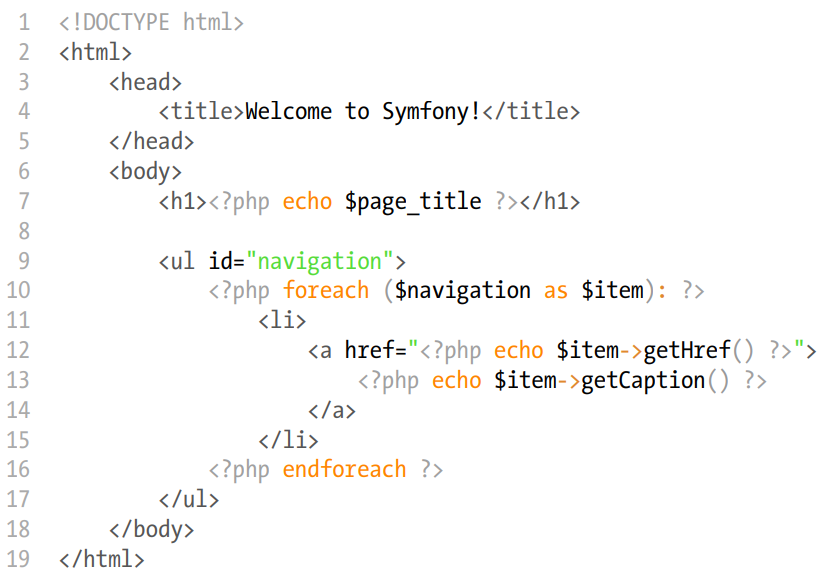
\includegraphics[width=0.68\textwidth]{twig-php.png}
        \end{center}
    \label{codeTemplatePHP}
    \legend{Fonte: \cite{symfonySensioLabs}}
\end{figure}

\bigskip

\begin{figure}[ht]
    \caption{Exemplo de \textit{template} em Twig .}
       	\begin{center}
            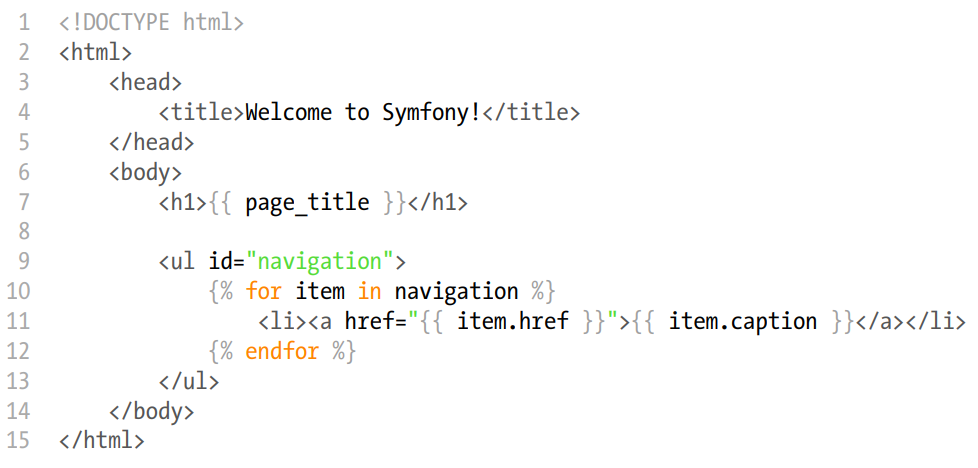
\includegraphics[width=0.68\textwidth]{figuras/twig-symf.png}
        \end{center}
    \label{codeTemplateTwig}
    \legend{Fonte: \cite{symfonySensioLabs}}
\end{figure}


\section{Projeto de Banco de dados}
\label{metodologiaBD}

A etapa final do projeto de banco de dados consiste na implementação do modelo lógico de acordo com as regras e definições do SGBD escolhido. Para a transcrição do modelo em tabelas MySQL, foi utilizado o módulo do phpMyAdmin que faz parte dos \textit{softwares} e recursos instalados junto à pilha XAMPP (ver seção \ref{implementacaoConfig}). Através dessa ferramenta, é possível realizar consultas e  operações no SGBD como criação, edição e remoção de tabelas e registros. A Figura \ref{projetoImagens} ilustra a interface do phpMyAdmin, que exibe informações sobre as tabelas do banco de dados.

\begin{figure}[h]
    \begin{adjustwidth}{-1in}{-.8in}
        \begin{center}
            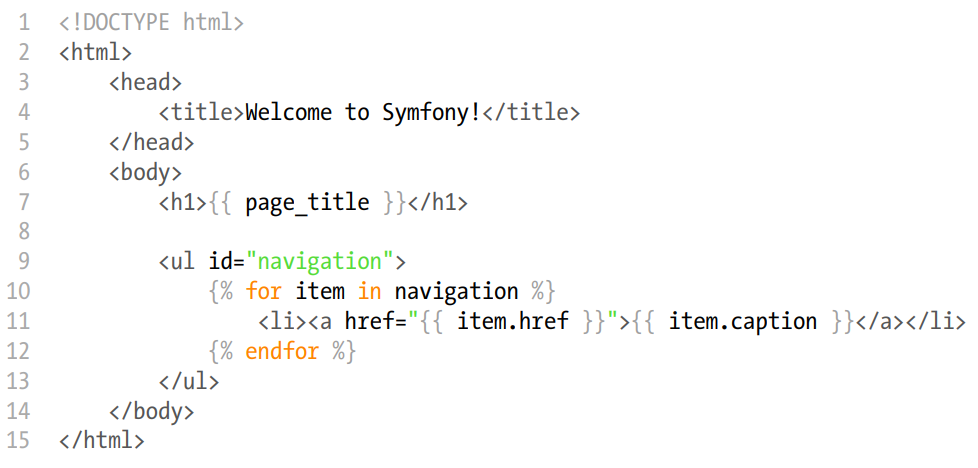
\includegraphics[width=0.68\textwidth]{figuras/twig-symf.png}
        \end{center}
        \caption{Telas para criação do banco de dados e configuração da tabela [nome tabela].}
        \label{projetoImagens}
    \end{adjustwidth}
\end{figure}

Ao final deste processo, a implementação do banco de dados da rede social foi concluído com 17 tabelas, sendo elas:

\begin{itemize}
    \item \textbf{block:} registra uma ação de bloqueio entre dois usuários, representado pelo campo "id\_blocker", correspondente ao usuário bloqueante, e "id\_blocked", usuário bloqueado. São armazenadas ainda a informação de quando ocorreu a ação pelo campo "datetime\_created"\ e se o bloqueio está ativo ainda, visto que é uma ação reversível, através do campo "active".
    
    \item \textbf{comment:} tabela que representa os comentários em postagens de usuários. Composta pelos campos "id\_author", que é o \textit{id} do usuário que fez o comentário; "id\_post", \textit{id} da postagem onde foi feito o comentário; "text", o conteúdo propriamente do comentário; "datetime\_published"\ e "datetime\_last\_edit"\ correspondem às datas de postagem e última edição respectivamente; "active", indica se o comentário está visível ou não (excluído).
    
    \item \textbf{favorite:} define a ação de favoritar uma vaga, representada pelos campos "id\_user, correspondente ao usuário que favorita, e "id\_job", à vaga favoritada. São armazenadas ainda a informação de quando ocorreu a ação pelo campo "datetime\_created"\ e se a vaga favoritada ainda está ativa, visto que é uma ação reversível, através do campo "active".
    
    \item \textbf{follow:} registra uma ação de seguir entre dois usuários, representado pelo campo "id\_follower", correspondente ao usuário seguidor, e "id\_following", usuário seguido. São armazenadas ainda a informação de quando ocorreu a ação pelo campo "datetime\_created"\ e se o ato de seguir está ativo ainda, visto que é uma ação reversível, através do campo "active".
    
    \item \textbf{job:} representa uma vaga divulgada no sistema. "id\_author"\ guarda o \textit{id} do usuário que criou a vaga; "title"\ é o título da vaga; "category\_list"\ é uma lista de \textit{id} de categorias da tabela \textit{job\_category} que determinam as áreas de atuação da vaga; "resume"\ é uma descrição breve da vaga ofertada e "text", o texto completo; "skills"\ é a lista de habilidades que são interessantes o candidato possuir; "type"\ é o tipo de vaga ofertada: pode ser 0 para Monitoria, 1 para Bolsa administrativa, 2 para Bolsa de iniciação científica, 3 para Estágio, 4 para Trainee, 5 para Efetivo ou 6 para Voluntário; "modality"\ é a modalidade da vaga: 0 corresponde a uma vaga Presencial, 1 à distancia; "salary"\ representa a remuneração mensal (em reais); "semester"\ indica a partir de qual semestre o candidato estaria apto para se candidatar; "shift"\ registra em qual(is)  turno(s) o candidato terá de trabalhar, "is\_prae"\ é um campo booleano e representa se a vaga, caso seja uma bolsa da UFRGS, é exclusiva para beneficiários PRAE ou não; os campos "date\_start"\ e "date\_finish"\ indicam o período de vigência da vaga; "workload"\ corresponde ao total de horas semanais exigida pela vaga; os campos "location", "location\_city"\ e "location\_state"\ determinam o endereço da vaga; "need\_curriculum"\ especifica se a vaga exige \textit{curriculum vitae} do candidato; "need\_historic", de maneira semelhante, especifica se a vaga exige histórico escolhar do candidato; "datetime\_publication"\ e "datetime\_last\_edit"\ sinalizam as datas e horários que a vaga foi publicada e editada pela última vez respectivamente; por fim, o campo "active"\ guarda a informação se a vaga está disponível ou foi excluída.
    
    \item \textbf{job\_apply:} armazena informações de quando um usuário manifesta interesse por uma vaga. O campo "id\_user"\ guarda o \textit{id} do usuário que realizou a ação e "id\_job", o \textit{id} da vaga em si. Adicionalmente, o campo "datetime\_created"\ registra a data e horário da ação e a coluna "active"\ indica se a manifestação de interesse está ativa ainda, pois o usuário pode desfazer sua ação.
    
    \item \textbf{job\_category:} essa tabela corresponde às áreas de atuação relacionadas a uma vaga. O campo "id"\ é utilizado como chave estrangeira para a lista presente em "category\_list"\ da tabela \textit{job}. 
    
    \item \textbf{log:} registra todas as ações relevantes que um usuário realizou no sistema. A tabela possui os seguintes campos e semântica: "id\_user"\ indica o \textit{id} do usuário que fez a ação; "type"\ define se a ação diz respeito a outro usuário, valor 1, ou a uma vaga, valor 2. O campo "action"\ é o código da ação relevante, podendo ser o valor desta: 1 para criação, 2 para atualização ou 3 para remoção de algum registro no sistema; 4, seguir usuário; 5, deixar de seguir usuário; 6, bloquear usuário; 7, desbloquear usuário; 8, candidatar-se a vaga; 9, aprovar candidato em vaga; 10, rejeitar candidato em vaga; 11, recomendar usuário; 12, recomendar vaga; 13, realizar uma postagem; 14, favoritar uma vaga; 15, desfavoritar vaga; 16, comentar em uma postagem; 17, realizar primeiro login no sistema; 18, atualizar foto de perfil; 19, curtir uma postagem. Por fim, o campo "datetime\_created"\ indica o horário e data de quando ocorreu a ação pelo usuário.
    
    \item \textbf{post:} armazena todas as informações de um post feito por um usuário. O campo "id\_author"\ indica o \textit{id} do usuário que fez a postagem; "text"\ é o conteúdo da postagem; "datetime\_published"\ e "datetime\_last\_edit"\ representam as datas de criação e última edição da postagem respectivamente; "privacy"\ restringe a exibição do \textit{post}: 1, somente o autor pode olhar ou 0, todos os usuários; "allow\_comments"\ caso possua o valor 1, qualquer usuário pode comentar na postagem, caso contrário, nenhum pode; "active"\ é um indicativo se o post está visível ou não (foi excluído pelo autor).
    
    \item \textbf{post\_like:} registra a curtida de um usuário em um post. Os campos criados para a tabela são: "id\_user", referente ao \textit{id} do usuário; "id\_post", que diz respeito ao \textit{id} do post; "datetime\_created"\ informa a data e horário que ocorreu a ação do usuário; "active"\ sinaliza se a curtida está ativa, uma vez que a ação pode ser desfeita.
    
    \item \textbf{recommendation\_job:} define a tabela que guarda informações sobre a recomendação de uma vaga. O campo "id\_user"\ indica o \textit{id} do usuário que fez a recomendação; "id\_job"\ é o \textit{id} da vaga recomendada; "text"\ corresponde ao conteúdo da recomendação, seu texto; os campos "datetime\_published"\ e "datetime\_last\_edit"\ representam as datas de criação e última edição da recomendação respectivamente; "active"\ é um indicativo se a recomendação está visível ou não (excluída pelo autor).
    
    \item \textbf{recommendation\_user:} define a tabela que armazena dados sobre a recomendação de um usuário. O campo "id\_user"\ indica o \textit{id} do usuário que fez a recomendação; "id\_target"\ é o \textit{id} do usuário recomendado; "text"\ corresponde ao conteúdo da recomendação, seu texto; os campos "datetime\_published"\ e "datetime\_last\_edit"\ representam as datas de criação e última edição da recomendação respectivamente; "active"\ é um indicativo se a recomendação está visível ou não (excluída pelo autor).
    
    \item \textbf{user:} tabela que salva todos os dados do usuário no sistema. É composta por: "name"\ representa o nome do usuário no sistema; "age"\ é a idade do usuário; "born\_in\_city"\ e "born\_in\_state"\ indicam a cidade e o estado do local de nascimento respectivamente; "live\_in\_city"\ e "live\_in\_state"\ indicam a cidade e o estado onde o usuário reside no momento. "role"\ é a função deste no sistema sendo o valor 1 para Administrador; 2, professor; 3, técnico; 4, aluno. "phone"\ é o seu telefone de contato principal; "birthday"\ sua data de nascimento; "gender", seu sexo onde 0 é Masculino e 1, Feminino; "personal\_link"\ é um campo para o usuário divulgar sua página pessoal através de um link na Internet; "avatar"\ guarda o caminho relativo da imagem utilizada como foto de perfil do usuário no sistema; "email\_notification"\ sinaliza a preferência do usuário para receber \textit{e-mails} de notificação do sistema; "show\_schollar\_info"\ e "show\_curriculum"\ são campos que, caso o usuário deseje, ele pode exibir as informações de histórico escolar e currículo no seu perfil respectivamente (valor 1 na coluna) ou omiti-los (valor 0); os campos "follower\_privacy"\ e "following\_privacy"\ restringem o acesso a informações sobre quem o usuário segue e quem o segue para usuários que não o seguem; "post\_privacy"\ é uma comodidade do sistema: indica a opção padrão durante criação de postagens; "datetime\_joined"\ salva a data de ingresso da primeira vez que o usuário fez \textit{login} no sistema. Este último e ainda os campos "id", "login", "email", "password"\ tiveram de ser simulados devido a restrições de integração do sistema (Ver seção \ref{redeLimitacao}).
    
    \item \textbf{user\_education:} relaciona um qualificação de ensino a um usuário. O campo "id\_user"\ é a chave estrangeira para o \textit{id} de um usuário na tabela \textit{user}. As colunas "title"\ e "subtitle"\ se referem ao grau de instrução ou informação de curso e a escola, universidade ou outra instituição de ensino onde o usuário estudou. "date\_start"\ e "date\_finish"\ guardam as informações do período que o usuário estudou na instituição. "location\_city"\ e "location\_state"\ mostram a cidade e o estado do ensino. O campo "selected"\ sinaliza se o trabalho é destaque; cada usuário pode destacar apenas uma qualificação para ser exibida em informações simplificadas de perfil. Ainda, "active"\ informa se o dado está ativo ou foi excluído.
    
    \item \textbf{user\_job:} relaciona uma experiência de trabalho a um usuário. O campo "id\_user"\ é a chave estrangeira para o \textit{id} de um usuário na tabela \textit{user}. As colunas "title"\ e "company"\ se referem ao cargo e empresa onde o  usuário trabalhou. "date\_start"\ e "date\_finish"\ guardam as informações do período que o usuário trabalhou na empresa. "location\_city"\ e "location\_state"\ mostram a cidade e o estado do trabalho. A coluna "selected"\ sinaliza se o trabalho é destaque; cada usuário pode destacar apenas um trabalho para ser exibido em informações simplificadas de perfil. Por fim, "active"\ informa se o registro está ativo ou foi excluído.
    
    \item \textbf{user\_language:} representa o conhecimento de um usuário sobre um idioma. O campo "title"\ é o idioma em questão. "level"\ indica o nível que o usuário possui, sendo 1 para Básico; 2, Intermediário; 3, Avançado; 4, Fluente; 5, Nativo. A coluna "active"\ informa se o dado está ativo ou foi excluído pelo usuário.
    
    \item \textbf{user\_skill:} representa o nível de proeficiência de um usuário sobre uma habilidade que ele possui. O campo "title"\ é a habilidade em questão. "level"\ indica o nível que o usuário possui, sendo 1 para Iniciante; 2, Amador; 3, Júnior; 4, Pleno; 5, Sênior. "time"\ indica o tempo (em anos) que o usuário possui essa habilidade. A coluna "active"\ informa se o dado está ativo ou foi excluído pelo usuário.
    
\end{itemize}

O apêndice \ref{appendDER} apresenta o diagrama entidade-relacionamento completo do projeto de banco do dados.

\section{Implementação}
\label{metodologiaImplementação}

A ferramenta foi implementada utilizando os conceitos de metodologia ágil de desenvolvimento com os \textit{frameworks} Scrum e Kanban. O desenvolvimento da aplicação foi dividido em cinco fases: construção do \textit{framework} da aplicação e  as entregas Inicial, Alfa, Beta e Final. Para uma maior organização durante toda a realização deste projeto, foi criado um repositório no GitHub\footnote{\url{https://github.com/jaflesch/tcc-ufrgs} Acesso em novembro de 2018}. Neste repositório, foram definidas várias \textit{issues}, que representavam as funcionalidades a serem implementadas no sistemas (analogamente, seriam um \textit{card} no quadro Kanban). Estas, agrupadas em \textit{milestones}, representavam um \textit{Sprint}, ou seja, uma etapa de desenvolvimento específico que deveria ser entregue em um período de duas semanas. A organização do quadro Kanban foi alcançada utilizando a ferramenta gratuita Trello\footnote{\url{https://trello.com/}, Acesso em novembro de 2018}.

\subsection{Configuração do ambiente do trabalho}
\label{implementacaoConfig}

Para instalar todas as ferramentas para execução da rede social, foi utilizada o pacote de código aberto XAMPP\footnote{\url{https://www.apachefriends.org/pt_br/index.html} Acesso em novembro de 2018.} que reúne todos os \textit{softwares} utilizados para criar um \textit{webserver} em um único computador, independente de sistema operacional.

A versão do XAMPP utilizada neste trabalho foi a 5.6.38, que inclui  Apache 2.4, PHP 5.6, MySQL 5.6,  e phpMyAdmin (entre outros recursos que não foram necessários à aplicação).

\subsection{\textit{Framework} do sistema}
\label{implementacaoFramework}

A construção do \textit{framework} focava em implementar conceitos abstratos da linguagem, arquiteturas do sistema e funcionalidades básicas que seriam reaproveitadas nas etapas seguintes, como roteamento das páginas, configuração da conexão ao banco de dados e métodos genéricos.

O padrão de arquitetura utilizado foi o MVC. Devido a flexibilidade e desacoplamento entre as camadas, foi adicionada uma lógica de roteamento no controlador. Basicamente, sempre que uma requisição HTTP chega ao servidor, existe um arquivo de configuração do Apache chamado \textit{.htaccess} que intercepta o pedido do cliente e o reescreve segundo as regras estipuladas. Neste caso, o objetivo é tornar amigáveis as URLs de acesso às páginas, isto é, deixá-las legíveis e organizadas. Para alcançar essa meta, toda requisição é enviada a uma variável \verb|$_GET['url']| do PHP e sempre é chamado o arquivo \textit{index.php} no diretório raiz.

A partir deste momento, a classe \verb|AppRouter| analisa o valor da variável e a fragmenta em duas partes principais: controlador e ação. O controlador é um nome da classe presente em arquivo de script PHP localizado na pasta "/\_controller/"\ e a ação é o nome do método invocado nesta classe. Por exemplo, se o usuário deseja acessar a página de vagas favoritas da aplicação, sua URL seria "/vagas/favoritos"\ e o roteamento instanciaria a classe \verb|Vagas|, presente no arquivo \textit{vagas.php}, e chamaria o método \verb|favoritos()|. 

Dentro do método invocado, são aplicados comandos para adicionar, editar ou simplesmente ler dados presentes no banco de dados. Essas chamadas são auxiliadas através das abstrações da camada de modelo do MVC. No sistema, elas estão definidas em classes, separadas por arquivos, dentro da pasta "/\_models/".

Por fim, dependendo do tipo de requisição submetida pelo usuário e do roteamento realizado, o controlador gerará uma visão que pode ser tanto um HTML puro, para carregar uma página nova, ou em formato JSON, quando é feita uma requisição AJAX no servidor. Quando a saída é em formato HTML, é invocado o método \verb|render()| cujos parâmetros são: caminho do arquivo de template do Twig e uma coleção de valores. A Figura \ref{codeFramework} exibe como é implementado no \textit{framework} o exemplo de vagas favoritas discutido previamente.

\begin{figure}[h]
    \caption{Exemplo de código utilizado no \textit{framework}: página de vagas favoritas é renderizada com as informações obtidas nos modelos \textit{Job} (vaga) e \textit{Profile} (perfil de usuário). }
       	\begin{center}
            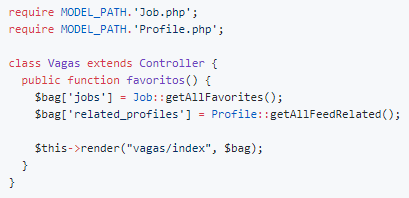
\includegraphics[width=.75\textwidth]{figuras/code-1.png}
        \end{center}
    \label{codeFramework}
    \legend{Fonte: Autor}
\end{figure}

O fluxo completo da requisição HTTP passando pela lógica de roteamento, pelas camadas de controlador e modelo do MVC, chegando ao banco de dados e retornando até a saída em HTML ou JSON na resposta HTTP pode ser observado na Figura \ref{routeFramework}.

\begin{figure}[h]
    \caption{ Funcionamento em alto nível da arquitetura MVC com a lógica de roteamento inserida.}
       	\begin{center}
            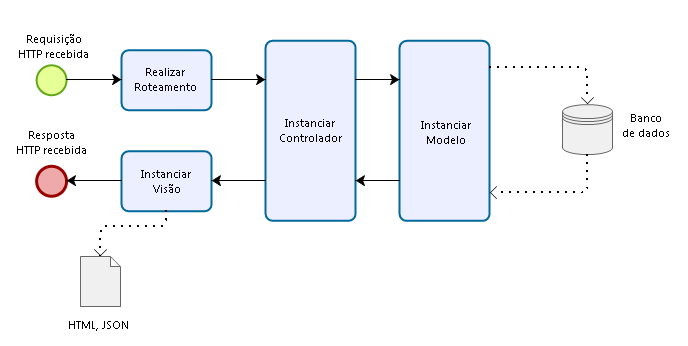
\includegraphics[width=0.9\textwidth]{figuras/roteamento.png}
        \end{center}
    \label{routeFramework}
    \legend{Fonte: Autor}
\end{figure}


\subsection{Versão Inicial}
\label{implementacaoIR}

A entrega inicial priorizou a elaboração das principais telas do sistema, como a páginas Inicial, Perfil de usuários, Vaga, Pesquisa e \textit{Login}. A funcionalidade de realizar autenticação no sistema também foi implementada nesta etapa junto com consultas ao banco de dados que exibiam informações parciais de entidades como usuário e vaga.

\subsection{Versão Alfa}
\label{implementacaoAR}

A segunda etapa destinou-se à interação entre os usuários. Ao término da entrega Alfa, já era possível seguir ou deixar de seguir um usuário, bloquear ou desbloquear um usuário, curtir ou descurtir um \textit{post} -e suas curtidas eram contabilizados dinamicamente-, favoritar ou desfavoritar vaga, recomendar um usuário ou vaga. 

Sobre os aspectos visuais, foram desenvolvidas as páginas restantes: Configurações gerais, Configurações de privacidade, Usuários bloqueados, Seguidores; a barra de menu lateral ficou funcional e com animações ao abrir e fechar. Melhorias na experiência de usuário foram aplicadas com o aumento da área de clique em botões e no uso de cores mais contrastantes.

\subsection{Versão Beta}
\label{implementacaoBR}

A entrega Beta trouxe diversas melhorias às funcionalidades desenvolvidas. A pesquisa de vagas e de usuários ganharam novos filtros de modo a tornar a sua utilização mais inteligente, dinâmica e eficiente. Além disso, a interação quando um usuário manifestava interesse por vaga e a posterior gerência por parte de quem a divulgou foi finalizada. Por fim, a biblioteca de envio de \textit{e-mails} para registrar e notificar ações importantes realizadas por usuários no sistema foi implementada.

No \textit{frontend}, iniciaram-se os primeiros passos para tratar as questões de responsividade em aparelhos móveis.

\subsection{Versão Final}
\label{implementacaoFR}

A última \textit{Sprint} do desenvolvimento teve três grandes focos: documentação de código e visual responsivo.  A parte operacional do sistema, isto é, as chamadas de funções e métodos, uso de classes e demais recursos propicionados pela linguagem PHP, no contexto do \textit{framework}, foram devidamente documentados. A intenção é de que, caso o sistema seja validado e utilizado no futuro, os desenvolvedores encarregados de incrementar o \textit{software} encontrem uma documentação completa e que a curva de aprendizagem das tecnologias utilizadas seja consideravelmente reduzida.

A visualização da rede social também foi concluída nesta etapa. Elementos restantes do \textit{layout} responsivo foram aplicados e isso possibilitou o uso da plataforma em dispositivo móveis sem comprometer a experiência do usuário. Pelo contrário, a disposição dos elementos foi ajustada para facilitar a interação e navegação pelo sistema.